\chapter{Adding user defined equation solver}

\modinfo{Directory}{Temperature1D}
\modinfo{Solvers}{\Idx{PoissonSolver}} 
%\modinfo{Files}{1dheat.grd, 1dheat.sif, Poisson.f90}
\modinfo{Tools}{Editor, \Idx{Fortran 90 compiler}, \Idx{ElmerGrid}}
\modinfo{Dimensions}{1D, Steady-state}

\subsection*{Problem description}

This tutorial is about creating the code for a simple poisson equation solver.
The solver is applied to 1d case with internal source term and fixed boundaries.

Mathematically the problem we solve is
\begin{equation}
\left \{
\begin{array}{cccc}
- \Delta \Phi &= &f & \mbox{ in } \Omega \\
\Phi&=&0 & \mbox{ on } \Gamma
\end{array}
\right .
\end{equation}

Allthough this example is in 1d the same solver code also applies to 2D and 3D
problems.

\subsection*{Solution procedure}

Own codes solving some specific equation may be added dynamically to Elmer 
software. Here we create a very simple equation solver code. The final code
may be found in the tutorial directory as well as the files for running
the example. The solution may be attempted as follows:

\begin{itemize}
\item Copy all the files from tutorial directory to current directory
\item Setup Elmer
\item Give the following commands:
\ttbegin
elmerf90 -o Poisson Poisson.f90
ElmerGrid 1 2 1dheat
ElmerSolver
ElmerPost
\ttend
\end{itemize}

\subsection*{The solver code}

The example Fortran code may be found in the tutorial files under the
name Poisson.f90.  The example run is defined in 1dheat.sif.
Only a rough guidline is given here of both of the files, refer to the
files themselves for more details.

All the  equation solvers in Elmer have the following common interface
\ttbegin
SUBROUTINE PoissonSolver( Model, Solver, dt, TransientSimulation )
  USE SolverUtils

  TYPE(Model) :: Model
  TYPE(Solver_t), POINTER :: Solver
  REAL(KIND=dp) :: dt
  LOGICAL :: TransientSimulation

    ...
END SUBROUTINE PoissonSolver
\ttend

The argument Model contains pointers to the whole definition of the Elmer run.
The argument Solver contains parameters specific to our equation solver.
The argument dt and TransientSimulation are the current timestep size, and a
flag if this run is steady or transient. These don't concern us this time.

When starting the ElmerSolver looks the solver input (.sif) file for a
Solver section with keyword "Procedure". This should contain reference to
the compiled code

\ttbegin
   Procedure = "Poisson" "PoissonSolver"
\ttend
where the first string in the right hand side is the file name of the compiled
code, and second argument is the name of the subroutine to look for in the given file.

In the Solver section one also gives the name of the field variable
(here Poisson) and the DOFs/node (here 1).

The basic duty of the equation solver is to solve one or more field variables inside
the time progressing- or steady state iteration-loop of ElmerSolver.  Here we use
FEM to discretize the Poisson equation and finally solve the equation by calling
ElmerSolver utility SolveSystem.

The solution progresses the following way:

\begin{itemize}
\item Get the space for variables and temporaries from ElmerSolver and compiler.
The matrix structure and space for solution and RHS vector have already been
allocated for you before you enter the equation solver.

The matrix is of type Matrix\_t and may be obtained from the arguments as
\ttbegin
TYPE(Matrix_t), POINTER :: StiffMatrix
StiffMatrix => Solver % Matrix
\ttend
Usually one doesn't need to know the internal storage scheme or the fields
of the Matrix type, but one just passes this pointer further to ElmerSolver
utility routines.

Similarly, the force vector may be accessed as follows:
\ttbegin
REAL(KIND=dp), POINTER :: ForceVector(:)
ForceVector => StiffMatrix % RHS
\ttend

The solution vector is obtainable similarily
\ttbegin
TYPE(Variable_t), POINTER :: Solution
Solution => Solver % Variable
\ttend

The Variable\_t structure contains the following fields
\begin{itemize}
\item DOFs: the number of degrees of freedom for one node. This value is for
information only and should'nt be modified.
\item Perm: an integer array that is nonzero for nodes that belong
to computational volume for this equation. The entry $Perm(i)$ holds
the index of the global matrix row  (for 1 DOF) for nodal point i.
This array  should'nt be modified by the equation solver.
\item Values: Space for the solution vector values.
Note that the values
are ordered the same way as the matrix rows, .i.e. the value of Potential at node
n is stored at
\ttbegin
  val = Solution % Values( Solution % Perm(n) )
\ttend
\end{itemize}


\item Initialize the global system to zero. Calling the utility routing
\ttbegin
CALL InitializeToZero( StiffMatrix, ForceVector )
\ttend
is usually enough.


\item Go trough the elements for which this equation is to 
be solved, get the elemental matrices and vectors and add them to
the global system:

\ttbegin
DO i=1,Solver % NumberOfActiveElements
   CurrentElement => Solver % Mesh % Elements( Solver % ActiveElements(i) )
      ...
   CALL LocalMatrix( ... )
   CALL UpdateGlobalEquations( ... )
END DO
CALL FinishAssembly( ... )
\ttend

Here the LocalMatrix is your own subroutine computing elemental matrices and vectors.
In the example code LocalMatrix uses three routines from ElmerSolver utilities. The function 
\ttbegin
  dim = CoordinateSystemDimension()
\ttend
returns the dimension of the current coordinate system, i.e. the return value is 
1, 2 or 3 depending on the input file setting of keyword "Coordinate System". The function
GaussPoints returns structure containing the integration point local coordinates and weights
\ttbegin
  TYPE(GaussIntegrationPoints_t) :: IntegStuff
  IntegStuff = GaussPoints( Element )
\ttend
The fields of the type GaussIntegrationPoints\_t are
\ttbegin
INTEGER :: n
REAL(KIND=dp) :: u(:), v(:), w(:), s(:)
\ttend
the integer value n is the number of points selected. The arrays u,v and w
are the local coordinates of the points, and the array s contains the weights
of the points. One may call the GaussPoints-routine with second argument,
\ttbegin
  IntegStuff = GaussPoints( Element, n )
\ttend
if the default number of integration points for given element is not suitable.

Inside the integration loop the function ElementInfo is called:
\ttbegin
   TYPE(Element_t), POINTER :: Element
   TYPE(Nodes_t) :: Nodes
   REAL(KIND=dp) :: U,V,W,detJ, Basis(n), dBasisdx(n,3), ddBasisddx(n,3,3)

   stat = ElementInfo( Element, Nodes, U, V, W, detJ,  &
        Basis, dBasisdx, ddBasisddx, .FALSE. )
\ttend
This routine returns determinant of the element jacobian (detJ), basis function values
(Basis(n)), basis function global derivative values (dBasisdx(n,3)), basis function second
derivative values ( ddBasisddx(n,3,3) ). The second derivatives are only computed if the
next logical flag is set to true. All the values are computed at the point U,V,W inside
element defined by structures Element and Nodes.

Refer to the code for more details.

\item Set boundary conditions. Here only dirichlet boundary conditions are used. These
may be set by using the utility routine SetDirichletBoundaries.

\item Solve the system by calling utility routine SolveSystem.
\end{itemize}


\begin{figure}
\begin{center}
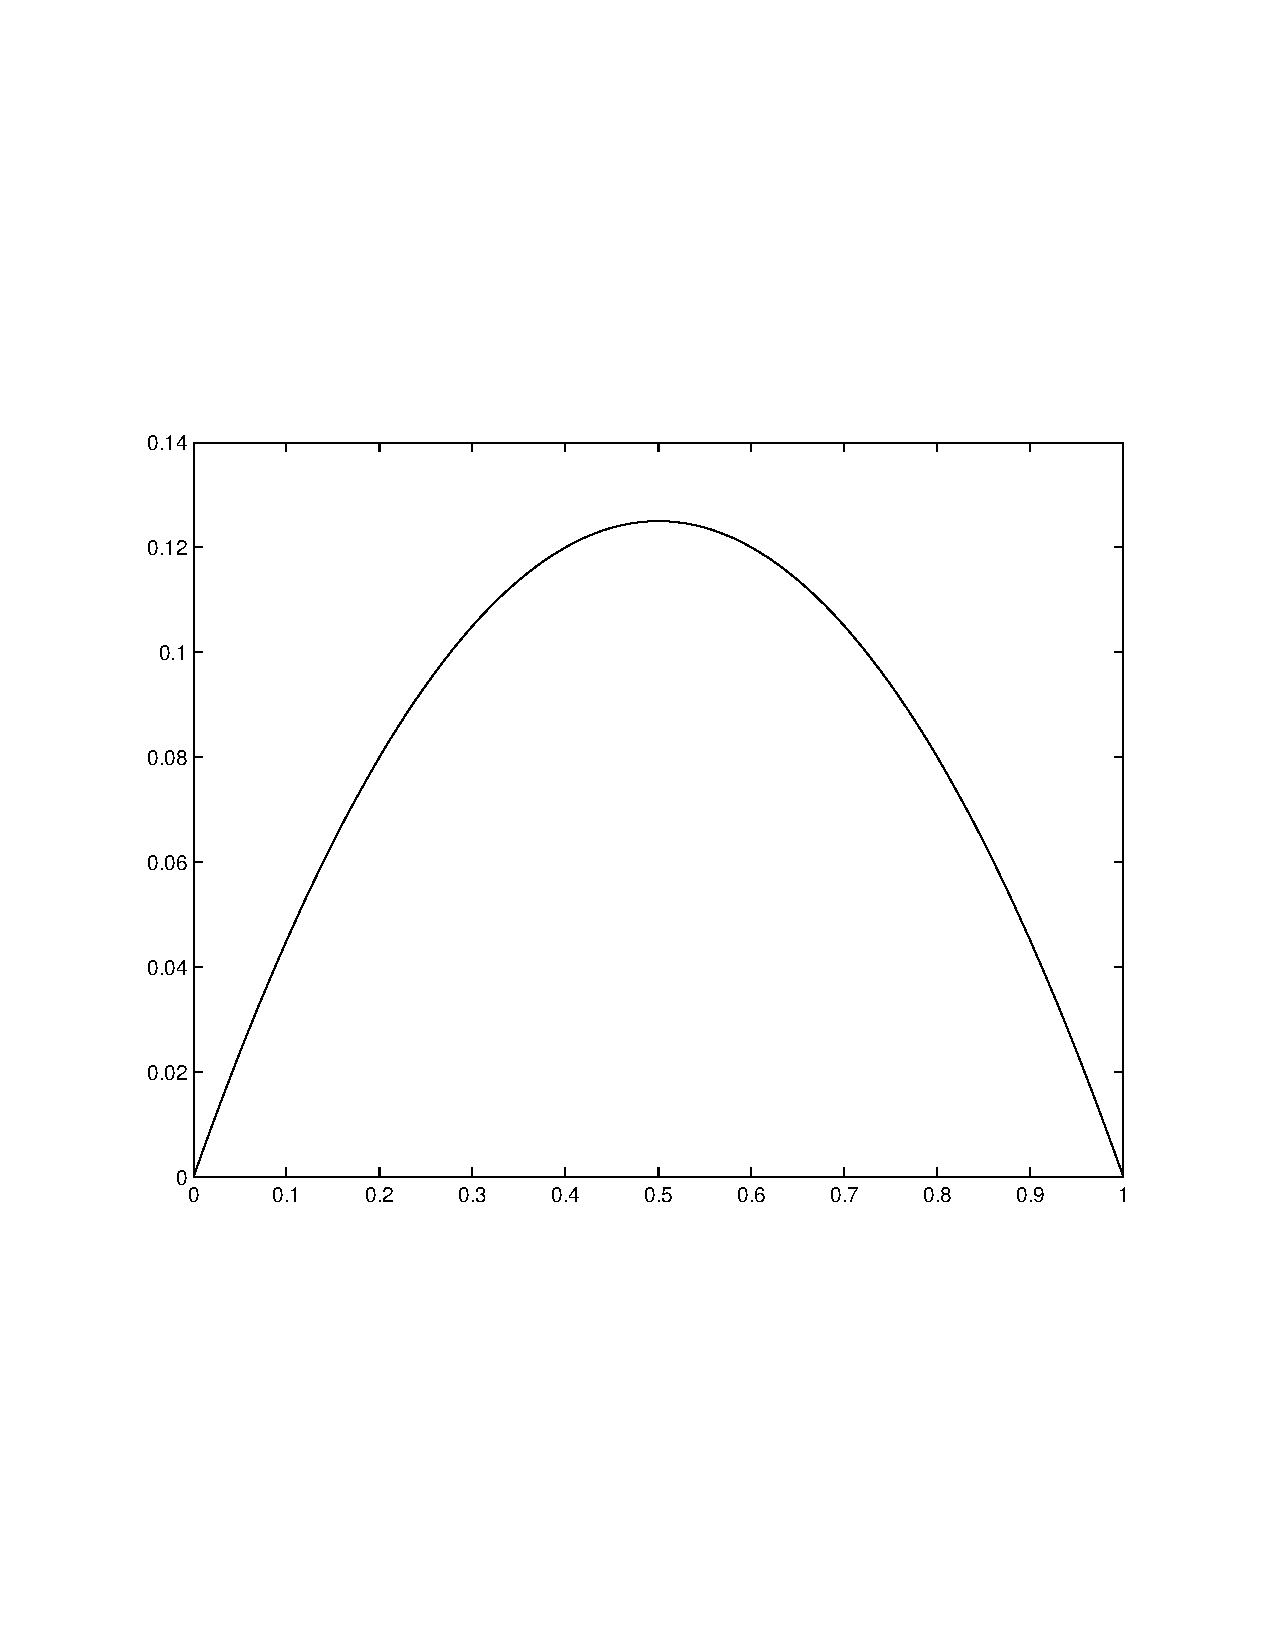
\includegraphics[width=0.6\textwidth]{1dheat}
\caption{Solution of the Poisson Equation.}\label{fg:pot}
\end{center}
\end{figure}
\subsection*{Results}

In the elmerpost file there is a variable called Potential which contains the
solution of this simple example. See figure~\ref{fg:pot}
